% Dmitry Mikushin, USI Lugano, dmitry.mikushin@usi.ch,
% using portions of original style file by Tom Cashman
%
% IMPORTANT NOTICE:
%
% The USI logo is unique; it is authorized for use only by employees of the
% Università della Svizzera italiana for work-related projects; others can use them
% ONLY with prior authorization (contact: press@usi.ch).
%
% http://www.press.usi.ch/en/corporate-design/corporate-design-stampa.htm
%
% This is an example beamer presentation, which uses Università della Svizzera italiana
% design theme.

\documentclass[aspectratio=169]{beamer}

\usetheme{usi}

\usepackage{multirow}
\usepackage{hhline}
\usepackage{tikz}
\usepackage{graphicx}
\usepackage{caption}
\captionsetup{compatibility=false}
\usepackage{subcaption}
\usepackage{listings}
\usepackage{array}
\usepackage{xcolor}
\usetikzlibrary{shapes.geometric}

\newcommand\score[2]{
\pgfmathsetmacro\pgfxa{#1+1}
\tikzstyle{scorestars}=[star, star points=5, star point ratio=2.25, draw,inner sep=1.3pt,anchor=inner point 3]
  \begin{tikzpicture}[baseline]
    \foreach \i in {1,...,#2} {
    \pgfmathparse{(\i<=#1?"usi@yellow":"gray")}
    \edef\starcolor{\pgfmathresult}
    \draw (\i*2.0ex,0) node[name=star\i,scorestars,fill=\starcolor,color=\starcolor]  {};
   }
  \end{tikzpicture}
}

\definecolor{cadmiumgreen}{rgb}{0.0, 0.42, 0.24}

\setlength{\fboxsep}{0.25pt}%
\setlength{\fboxrule}{0pt}%

\title[\textsc{\scriptsize heat-2d} on K40c with PPCG and PGI OpenACC]{\textsc{\huge heat-2d} performance on K40c with PPCG and PGI OpenACC}
\author{Olaf Schenk, Dmitry Mikushin}
\date{\today}


\begin{document}
\begin{frame}
\titlepage
\end{frame}



\begin{frame}[fragile]{Benchmark configuration}

\begin{itemize}
\item NVIDIA K40c on tesla-cmc
\item PPCG fa4e683fb467eb5d89733b3dd1e638a9d050968a
\item LLVM c59decb902128c7b68baf98f5eadcf26fbfa5a08
\item PGI OpenACC 15.7-0 64-bit
\item NVIDIA CUDA 7.0, V7.0.27
\end{itemize}

\end{frame}



\begin{frame}[fragile]{Benchmark performance results}

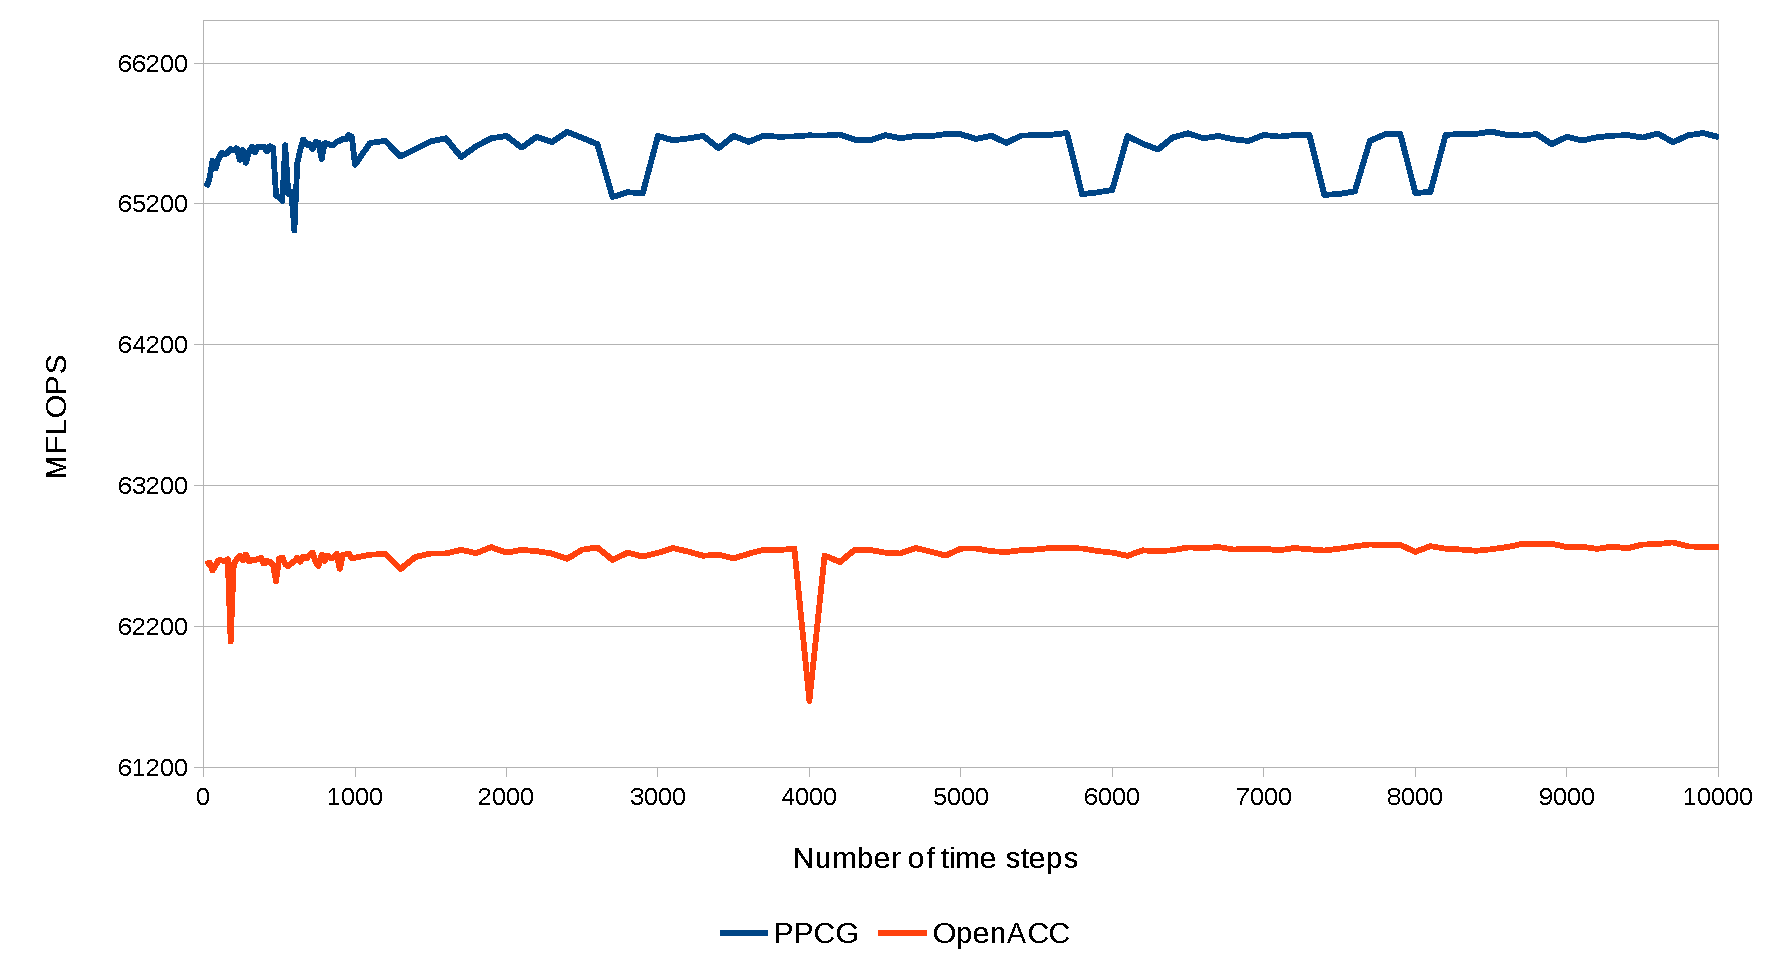
\includegraphics[width=13cm]{figures/tesla_k40}

\end{frame}



\begin{frame}[fragile]{Benchmark accuracy results}

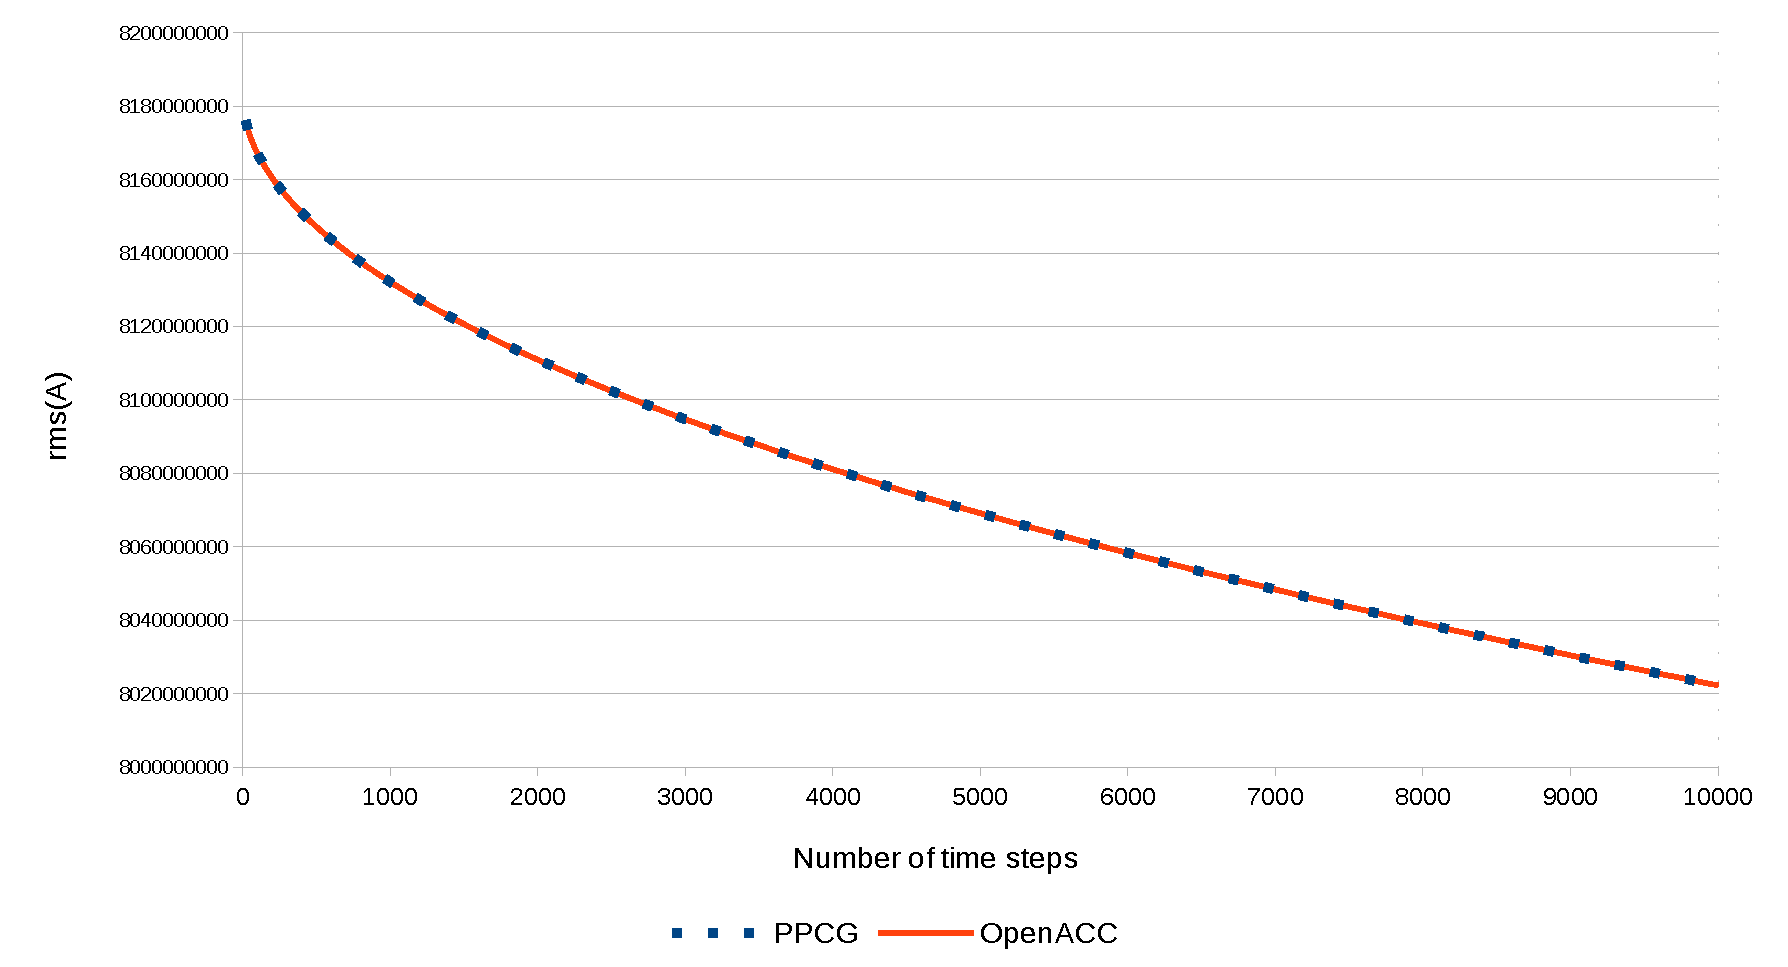
\includegraphics[width=13cm]{figures/tesla_k40_rms}

\end{frame}



\begin{frame}[fragile]{Profiling: Memory VS Compute}

\begin{minipage}{7cm}
\centering
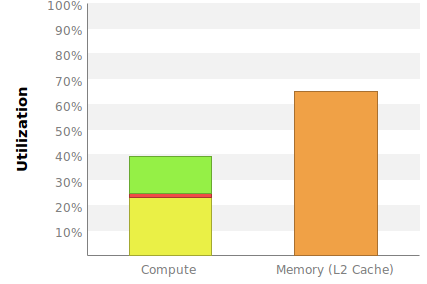
\includegraphics[height=4cm]{figures/ppcg_compute}\\
{\footnotesize PPCG}
\end{minipage}%
\begin{minipage}{7cm}
\centering
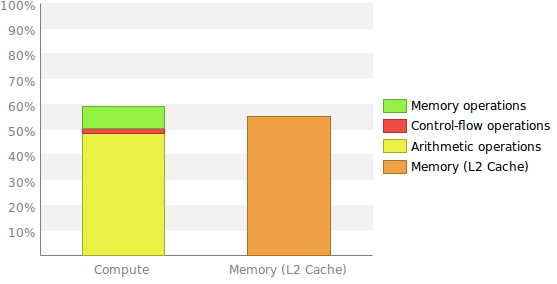
\includegraphics[height=4cm]{figures/openacc_compute}\\
{\footnotesize OpenACC}
\end{minipage}

\end{frame}



\begin{frame}[fragile]{Profiling: instructions}
\vskip10pt
\begin{minipage}{10cm}
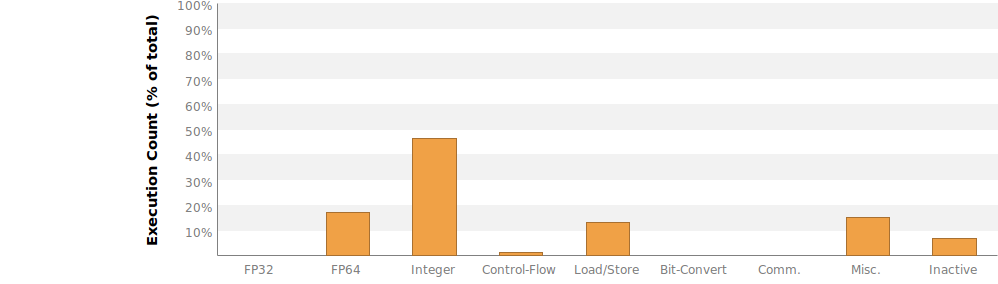
\includegraphics[height=2.9cm]{figures/ppcg_instructions}
\end{minipage}%
\begin{minipage}{2cm}
\hskip2cm
\end{minipage}%
\begin{minipage}{1cm}
{\footnotesize PPCG}
\end{minipage}
\vskip15pt
\begin{minipage}{10cm}
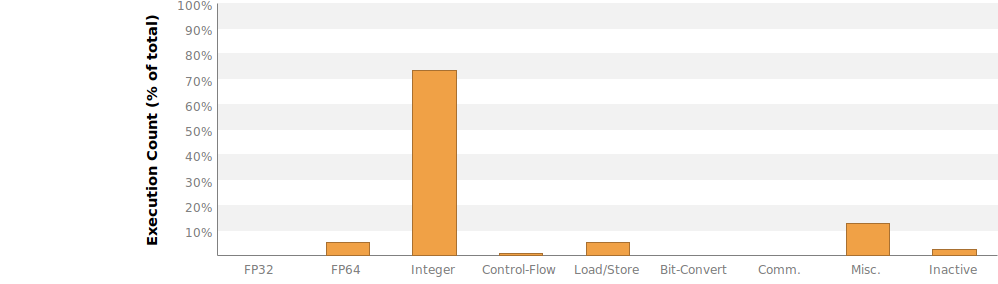
\includegraphics[height=2.9cm]{figures/openacc_instructions}
\end{minipage}%
\begin{minipage}{2cm}
\hskip2cm
\end{minipage}%
\begin{minipage}{1cm}
{\footnotesize OpenACC}
\end{minipage}

\end{frame}



\begin{frame}[fragile]{Profiling: Memory throughput}

\centerline{
\begin{minipage}[t]{3cm}
\centering
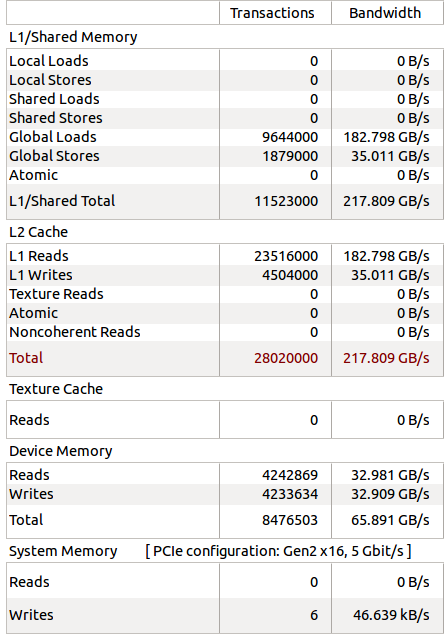
\includegraphics[height=6cm]{figures/ppcg_memory}\\
{\footnotesize PPCG}
\end{minipage}%
\begin{minipage}{0.5cm}
\hskip0.5cm
\end{minipage}%
\begin{minipage}[t]{4cm}
\centering
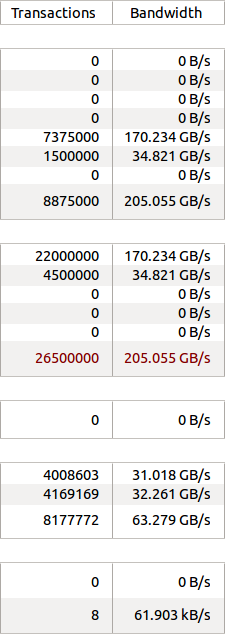
\includegraphics[height=6cm]{figures/openacc_memory}\\
{\footnotesize OpenACC}
\end{minipage}
}

\end{frame}



\begin{frame}[fragile]{Profiling: Memory throughput}

\centerline{
\begin{minipage}[t]{5cm}
\centering
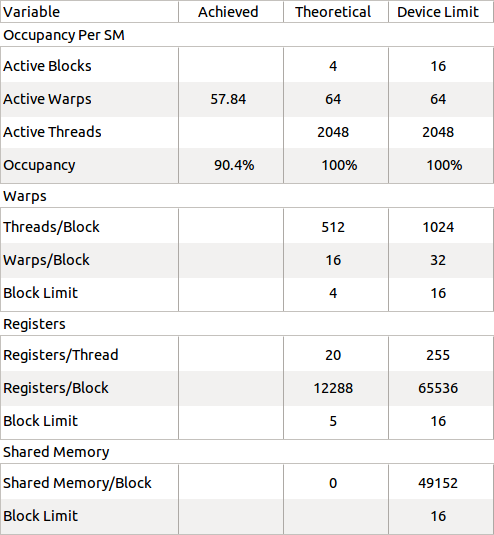
\includegraphics[height=6cm]{figures/ppcg_latency}\\
{\footnotesize PPCG}
\end{minipage}%
\begin{minipage}{0.5cm}
\hskip0.5cm
\end{minipage}%
\begin{minipage}[t]{4cm}
\centering
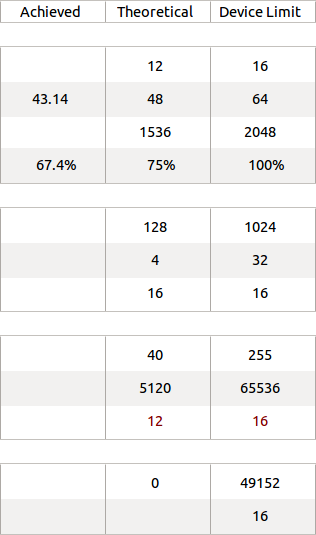
\includegraphics[height=6cm]{figures/openacc_latency}\\
{\footnotesize OpenACC}
\end{minipage}
}

\end{frame}



\begin{frame}[fragile]{Conclusion}

\begin{itemize}
\item PPCG outperforms OpenACC by 4\% with identical results
\item PPCG chooses grid configuration resulting into better occupancy
\end{itemize}

\end{frame}

\end{document}
